\documentclass[border=1pt]{standalone}
\usepackage[T1]{fontenc}
\usepackage{mathptmx}
\usepackage{tikz}
\usetikzlibrary{arrows.meta,positioning}
\begin{document}
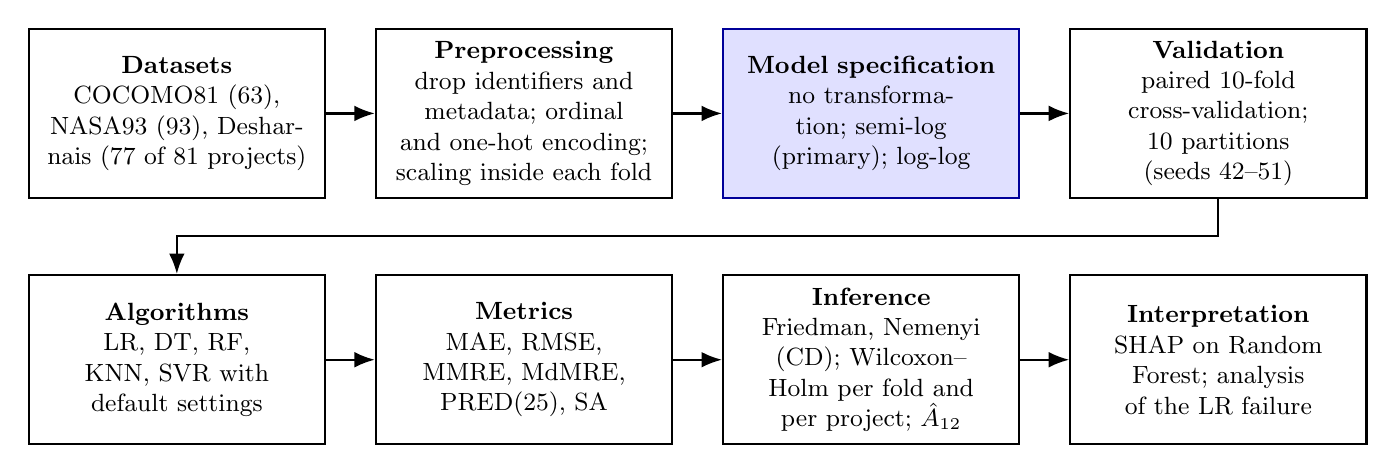
\begin{tikzpicture}[
  box/.style={draw, line width=0.8pt, align=center, text width=3.55cm, minimum height=2.15cm, inner sep=3pt, font=\small},
  arr/.style={-{Latex[length=2.6mm,width=2mm]}, line width=0.8pt},
  node distance=0.62cm]
\node[box] (d) {\textbf{Datasets}\\ COCOMO81 (63), NASA93 (93), Desharnais (77 of 81 projects)};
\node[box, right=of d] (p) {\textbf{Preprocessing}\\ drop identifiers and metadata; ordinal and one-hot encoding; scaling inside each fold};
\node[box, right=of p, fill=blue!12, draw=blue!60!black] (s) {\textbf{Model specification}\\ no transformation; \mbox{semi-log} (primary); log-log};
\node[box, right=of s] (v) {\textbf{Validation}\\ paired 10-fold \mbox{cross-validation}; 10~\mbox{partitions} (seeds 42--51)};
\node[box, below=0.95cm of d] (a) {\textbf{Algorithms}\\ LR, DT, RF, KNN, SVR with default settings};
\node[box, right=of a] (m) {\textbf{Metrics}\\ MAE, RMSE, MMRE, MdMRE, PRED(25), SA};
\node[box, right=of m] (i) {\textbf{Inference}\\ Friedman, Nemenyi (CD); Wilcoxon--Holm per fold and per project; $\hat{A}_{12}$};
\node[box, right=of i] (t) {\textbf{Interpretation}\\ SHAP on Random Forest; analysis of the LR failure};
\draw[arr] (d) -- (p); \draw[arr] (p) -- (s); \draw[arr] (s) -- (v);
\draw[arr] (a) -- (m); \draw[arr] (m) -- (i); \draw[arr] (i) -- (t);
\draw[arr] (v.south) -- ++(0,-0.47) -| (a.north);
\end{tikzpicture}
\end{document}
